\documentclass{standalone}

% Fontspec fot XeLaTeX
\usepackage{fontspec}
	% Unicode fonts
	\setmainfont{CMU Serif}

\usepackage{unicode-math}

\usepackage{tikz}
\usetikzlibrary{decorations.pathmorphing}
\usetikzlibrary{calc}

\newcommand{\rSch}{R_\text{S}} % Schwarzschild radius
\usepackage{amsmath}

\begin{document}
\begin{tikzpicture}%[scale=2]
\pgfmathsetmacro\myunit{3} 
	\draw (0,0)
			node [above] {$i^+$}
		--++(-45:\myunit)
			node [right] {$i^0$}
		--++(-135:\myunit)
			coordinate (b)
			node [below] {$i^-$};
	\draw [dashed] (b) -- (0,0);
\end{tikzpicture}

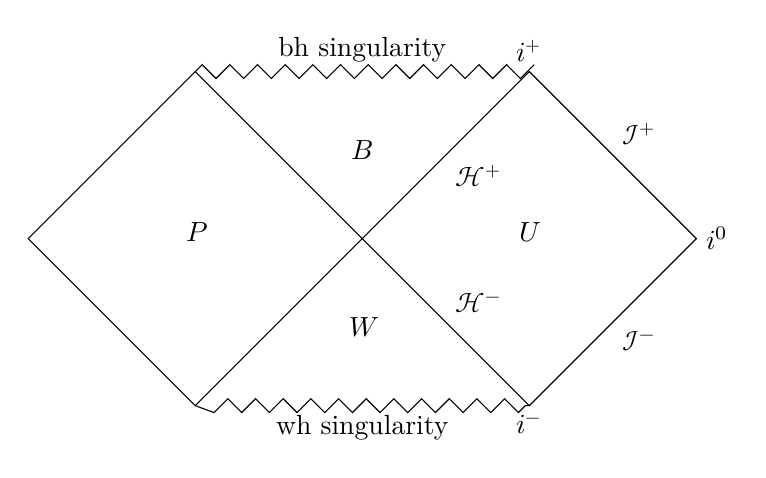
\begin{tikzpicture}%[scale=2]
\pgfmathsetmacro\myunit{3} 
	\draw (0,0)
			% node [left] {$i^0$} 
		--++(45:\myunit)
			% node [above]{$i^+$}
			coordinate (a)
			node [below = 1.8 cm] {$P$}
			% node [pos = .5, above left] {$\mscrI^+$}
			% node [pos=.5, below, sloped] {$\bar{u}=\infty$}
		--++(-45:2*\myunit)
			% node [pos = .25, above right] {$\mscrH^+$}
			node [pos = .75, above right] {$\mscrH^-$} %, sloped]{$r = \rSch$}%x_+ \to -\infty$}
			coordinate (d)	
			node [below]{$i^-$}
		--++(45:\myunit)
			node [pos = .5, below right] {$\mscrI^-$} % , sloped]{$x_- \to -\infty$}
			node [right] {$i^0$}
		--++(135:\myunit)
			node [pos = .5, above right] {$\mscrI^+$} % , sloped]{$x_+ \to +\infty$}
			node [above] {$i^+$}
			node [below = 1.8 cm] {$U$}
			coordinate (b)
		--++(-135:2*\myunit)
			coordinate (c)
			% node [pos = .25, below, sloped] {$r = \rSch$}%x_- \to +\infty$}
			% node [pos = .75, below right] {$\mscrH^-$}
			node [pos = .25, below right] {$\mscrH^+$}
			% node [below] {$i^-$}
		--cycle
			% node [pos = .5, below left] {$\mscrI^-$}
			;

	\draw [decorate, decoration=zigzag]
		(a) --
			node [above] {bh singularity} % =6pt
			node [below = .75 cm] {$B$}
			(b) 
		(c) --
			node [below] {wh singularity}
			node [above = .75 cm] {$W$}
			(d);

\end{tikzpicture}

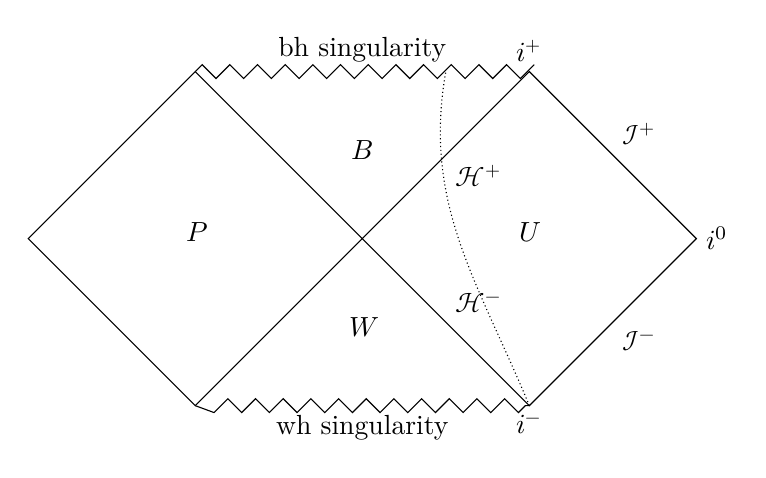
\begin{tikzpicture}%[scale=2]
\pgfmathsetmacro\myunit{3} 
	\draw (0,0)
			% node [left] {$i^0$} 
		--++(45:\myunit)
			% node [above]{$i^+$}
			coordinate (a)
			node [below = 1.8 cm] {$P$}
			% node [pos = .5, above left] {$\mscrI^+$}
			% node [pos=.5, below, sloped] {$\bar{u}=\infty$}
		--++(-45:2*\myunit)
			% node [pos = .25, above right] {$\mscrH^+$}
			node [pos = .75, above right] {$\mscrH^-$} %, sloped]{$r = \rSch$}%x_+ \to -\infty$}
			coordinate (d)	
			node [below]{$i^-$}
		--++(45:\myunit)
			node [pos = .5, below right] {$\mscrI^-$} % , sloped]{$x_- \to -\infty$}
			node [right] {$i^0$}
		--++(135:\myunit)
			node [pos = .5, above right] {$\mscrI^+$} % , sloped]{$x_+ \to +\infty$}
			node [above] {$i^+$}
			node [below = 1.8 cm] {$U$}
			coordinate (b)
		--++(-135:2*\myunit)
			coordinate (c)
			% node [pos = .25, below, sloped] {$r = \rSch$}%x_- \to +\infty$}
			% node [pos = .75, below right] {$\mscrH^-$}
			node [pos = .25, below right] {$\mscrH^+$}
			% node [below] {$i^-$}
		--cycle
			% node [pos = .5, below left] {$\mscrI^-$}
			;

	\draw [decorate, decoration=zigzag]
		(a) --
			node [above] {bh singularity} % =6pt
			node [below = .75 cm] {$B$}
			(b) 
		(c) --
			node [below] {wh singularity}
			node [above = .75 cm] {$W$}
			(d);

	\draw [densely dotted, out = 112.5, in = -100] (d)
		to ($(a)!0.75!(b)$);
\end{tikzpicture}

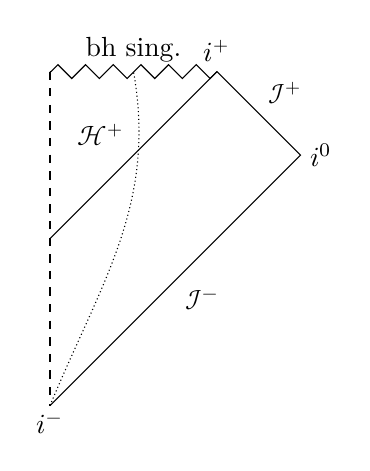
\begin{tikzpicture}%[scale=2]
\pgfmathsetmacro\myunit{3} 
\pgfmathsetmacro\sc{1.414213562} 
	\draw [dashed] (0,0)
		-- ++(-90: \sc * \myunit)
			node [below] {$i^-$}
			coordinate (a);
	\draw (a)
		-- ++(45: 1.5 * \myunit)
			node [right] {$i^0$}
			node [pos = .5, below right] {$\mscrI^-$}
		-- ++(135: 0.5 * \myunit)
			node [above] {$i^+$}
			node [pos = .5, above right] {$\mscrI^+$}
			coordinate (b)
		-- ++(-135: \myunit)
			node [pos = .5, above left] {$\mscrH^+$};
	\draw [decorate, decoration=zigzag] (b)
		-- (0,0)
			node [pos = .5, above] {bh sing.};
	\draw [densely dotted, out = 67.5, in = -80] (a)
		to (\sc/4* \myunit, 0);
\end{tikzpicture}
\end{document}